\chapter{Introduction}
In the first part of the manuscript, we show that direct reinforcement learning of decision tree policies for MDPs is often very difficult compared to indirect imitation of a neural network policy with a decision tree.

This first part of the manuscript is organised as follows.
In this chapter we present Topin et. al. formal framework for direct reinforcement learning of decision tree policies (cite).
In chapter (cite), we reproduce experiments from Topin et. al. where we compare direct deep reinforcement learning of decision tree policies to indirect imitation of a neural networf policy with a decision tree for the simple CartPole MDP.
In chapter (cite), we show that the direct approach proposed by Topin et. al. is equivalent to learning deterministic memoryless policy for partially observable MDPs (POMDPs) which is way more difficult that learning the same policies MDPs.
In chapter (cite), we show that when doing direct reinforcement learning of decision tree policies for MDPs which transitions are uniform, e.g. when the MDPs encode classification or regression tasks (cite), those POMDP problems are easy to solve. 

\section{Learning Decision Tree policies for MDPs}
There already exist algorithms that return decision tree policies for MDPs.
Those algorithms either learn parametric trees or non-parametric trees.

Parametric trees are not ``grown'' from the root by iteratively adding internal or leaf nodes depending on the interpretability-performance trade-off to optimize, but are rather ``optimized'': the depth, internal nodes arrengement, and state-features to consider in each nodes are fixed \textit{a priori} and only the tested thresholds of each nodes are optimized similarly to how the weights of a neural network are optimized.
As the reader might have guessed, those parametric trees are advantageous in that they can be learned with gradient descent and in the context of decision tree policies, with the policy gradient (cite).
The downside of those approaches is that a user cannot know \textit{a priori}  what a ``good'' tree policy structure should be for a particular MDP: either the specified structure is too deep and pruning will be required after training or the tree structure is not expressive enough to encode a good policy. 
Similar approaches exist in supervised learning exist where a parametric tree is fitted with gradient descent (cite). However their benefit over non-parametric trees have not been shown.
When parametric trees are learned for MDPs; extra stabilizing tricks are required during training such as adaptive batch sizes (cite).
Non-parametric trees are the standard model in supervised learning (cite) and can naturally trade-off between interpretability and performances. 
However, specialized approaches are required since growing a tree from the root in an RL fashion is not possible.
Recall that interpretable machine learning algorithms are either indirect.
In the introduction (cite), we showed that indirect imitation learning of neural network experts can lead to sub-optimal decision tree policies in terms of the RL objective (cite) because those trees optimize a surrogate imitation loss rather than the RL objective directly.

In 2021, Topin et. al. introduced iterative bouding Markov decision processes (IBMDPs) (cite). 
Given an MDP for which one wants to learn a decision tree policy, IBMDPs are an augmented version of this base MDP with more state features, more actions, additional rewards and additional transitions.
Authors showed that certain IBMDP policies, that can be learned \textit{directly} with RL, are equivalent to decision tree policies for the base MDP.

There also exists more specialized approaches that can return decision tree policies only for small problem classes.
In (cite), authors prove that for maze-like MDPs, there always exist an optimal decision tree policy and provide an algorithm to find it. 
In (cite), authors give an algorithm to return decision tree policies for MDPs that are constrained to have depth less than 3. 
Finally, in (cite), authors study decision tree policies for planning in MDPs, i.e., when the transitions and rewards are known.
In the next section we present IBMDPs as introduced in (cite).

\section{Iterative Bounding Markov Decision Processes}

The key thing to know about IBMDPs is that they are, as their name suggests, MDPs.
Hence, IBMPDs inherit MDPs properties such as existence of an optimal deterministic Markovian policy for problem (cite).
The states in an IBMDP are concatenations of the base MDP states and some observations. Those observations are information about the base states that are refined--``iteratively bounded''-- at each step and represent a subspace of the base MDP state space.
Actions available in an IBMDP are the actions of the base MDP, that change the state of the latter, and \textit{information gathering} actions that change the observation part of the IBMDP state.
Now, taking base actions in an IBMDP is rewarded like in the base MDP, this ensures that the base objective, e.g. balancing the pole or treating cancer, is still encoded in the IBMDP reward. When taking an information gathering action, the reward is an arbitrary value supposed to balance performance and interpretability.
 
Before showing how to get decision tree policies from IBMDP policies, we give a formal definition of IBMDPs following Topin et. al. (cite).

\begin{definition}[Iterative Bounding Markov decision process]
Given a \textit{factored} (cite) MDP $\mathcal{M}$ (cite) $\langle S, A, R, T, T_0 \rangle$, an associated Iterative Bouding MDP $\mathcal{M}_{IB}$ is a tuple:
\begin{align*}
    \langle \overbrace{S \times O}^{\text{State space}}, \underbrace{A \cup A_{info}}_{\text{Action space}}, \overbrace{(R, \zeta)}^{\text{Reward function}}, \underbrace{(T_{info}, T, T_0)}_{\text{Transitions}}\rangle
\end{align*}

\begin{itemize}
\item $S$ the base MDP factored state space. A state $\boldsymbol{s} = (s_1, \dots, s_n)\in S$ has $n$ bounded features $s_i \in [L_i, U_i]$ where $\infty < L_i \leq U_i < \infty \forall 1\leq i \leq n$.
\item $O$ are the observations in an IBMDP. They are partial information about the base MDP state features. The set of observations is the bounds of the state features bounds: $O\subsetneq S^2 =  [L_1, U_1]\times \dots \times [L_n, U_n] \times [L_1, U_1]\times \dots \times [L_n, U_n]$. So the complete IBMDP state space is $S \times O$ the concatenations of state features and observations.
\item $A$ is the base MDP actions set.
\item $A_{info}$ are \textit{information gathering} actions (IGAs) of the form $\langle i, v \rangle$ where $i$ is a state feature index $1 \leq i \leq n$ and $v$ is a real number. So the complete action space of an IBMDP is the set of base MDP actions and information gathering actions $A \cup A_{info}$.
\item $R: S\times A \rightarrow \mathbb{R}$ is the base MDP reward function that maps base states and actions to a real-valued reward signal.
\item $\zeta$ is a reward signal for taking an information gathering action. So the IBMDP reward function is to get a reward from the base MDP if the action is a base MDP action or to get $\zeta$ if the action is an IGA action.
\item $T_{info}: S\times O \times( A_{info} \cup A )\rightarrow \Delta (S\times O)$ is the transition kernel of IBMDPs: 
Given some observation $\boldsymbol{o}_t = (L'_1, U'_1, \dots, L'_n, U'_n) \in O$ and state features $\boldsymbol{s}_t=(s'_1, s'_2, \dots, s'_n)$ if an IGA $\langle i, v \rangle$ is taken, the new observation is:
\begin{align*}
    \boldsymbol{o}_{t+1} &= \begin{cases}
        (L'_1, U'_1, \dots , L'_i, \min\{v, U'_i\}, \dots , L''_n, U'_n) \text{ if } s_i \leq v\\
        (L'_1, U'_1, \dots , \max\{v, L'_i\}, U'_i, \dots , L''_n, U'_n) \text{ if } s_i > v
    \end{cases}
\end{align*}
If a base action $a_t\in A$ is taken, the new observation is the default state bounds $(L_1, U_1,\dots, L_n, U_n)$ and the state features change according to the base MDP transitition kernel: $\boldsymbol{s}_{t+1}\sim T(\boldsymbol{s}_t, a_t)$.
At initialization, the base state features are drawn from the base MDP $T_0$ and the observation is always set to the default state features bounds $\boldsymbol{o}_0=(L_1, U_1,\dots, L_n, U_n)$.
\end{itemize}
\end{definition}

Now remains to extract a decision tree policy for MDP $\mathcal{M}$ from a policy for an associated IBMDP $\mathcal{M}_{IB}$. 

\subsection{From Policies to Trees}

One can notice that information gathering actions resemble the Boolean functions that make up internal decision tree nodes (cite).
Indeed, a policy taking actions in an IBMDP essentially builds a tree by taking sequences of IGAs (internal nodes) and then a base action (leaf node) and repeats this process over time.

However, authors from (cite) show that not all IBMDP policies are decision tree policies.
In particular they show that only deterministic policies depending solely on the observation part of the IBMDP states are guaranteed to correspond to decision tree policies for the base MDP.

\begin{proposition}[Deterministic partially observable IBMDP policies are decision trees] 
    Given an IBMDP $\mathcal{M}_{IB} $ $ \langle S \times O,A \cup A_{info}, (R, \zeta), (T_{info}, T, T_0)\rangle$ a deterministic partially observable policy $\pi_{po}: O \rightarrow A\cup A_{info}$ is a decision tree policy $\pi_{\mathcal{T}}: S \rightarrow A$ for the base factored MDP $\langle S, A, R, T, T_0\rangle$ (cite).
\end{proposition}
\begin{proof}(Sketch) Algorithm (cite) that takes as input a deterministic partially observable policy $\pi_{po}$ for an IBMDP $\mathcal{M}_{IB}$ $\langle S \times O,A \cup A_{info}, (R, \zeta), (T_{info}, T, T_0)\rangle$, returns a decision tree policy $\pi_{\mathcal{T}}$ for $\mathcal{M}=\langle S, A, R, T, T_0\rangle$ and always terminates unless the deterministic partially observable policy only takes IGAs.
\end{proof}

\begin{algorithm}[t]
    \KwData{Deterministic partially observable policy $\pi_{po}$ for IBMDP $ \langle S \times O,A \cup A_{info}, (R, \zeta), (T_{info}, T, T_0)\rangle$ and observation IBMDP $\boldsymbol{o}=(L'_1, U'_1, \dots, L'_n, U'_n)$}
    \KwResult{Decision tree policy $\pi_{\mathcal{T}}$ for MDP $\langle S, A, R, T, T_0\rangle$}
    
    \SetKwProg{Fn}{Function}{:}{}
    \SetKwFunction{SubtreeFromPolicy}{Subtree\_From\_Policy}
    
    \Fn{\SubtreeFromPolicy{$\boldsymbol{o}, \pi_{po}$}}{
        $a \leftarrow \pi_{po}(\boldsymbol{o})$ \\
        \If{$a \in A_{info}$}{
            \Return Leaf\_Node(action: $a$) \Comment{// Leaf if base action}
        }
        \Else{
            $\langle i, v\rangle \leftarrow a$ \Comment{// Splitting action is feature and value} \\
            $\boldsymbol{o}_L \leftarrow \boldsymbol{o}; \quad \boldsymbol{o}_R \leftarrow \boldsymbol{o}$ \\
                         $\boldsymbol{o}_L \leftarrow (L'_1, U'_1, \dots, L'_i, v, \dots, L'_n, U'_n); \quad \boldsymbol{o}_R \leftarrow (L'_1, U'_1, \dots, v, U'_i, \dots, L'_n, U'_n)$ \\
            $child_L \leftarrow$ Subtree\_From\_Policy$(\boldsymbol{o}_L, \pi_{po})$ \\
            $child_R \leftarrow$ Subtree\_From\_Policy$(\boldsymbol{o}_R, \pi_{po})$ \\
            \Return Internal\_Node(feature: $i$, value: $v$, children: $(child_L, child_R)$)
        }
    }
    
    \caption{Extract a Decision Tree Policy}\label{alg_extract_tree}
\end{algorithm}

We defer the connexions with POMDPs to Chapter (cite).

\subsection{Example: an IBMDP for a grid world}
Suppose a factored MDP representing a grid world with 4 cells like in Example (cite). 
The states are the $(x,y)$-cooridnates $S = \{(0.5, 0.5), (0.5, 1.5), (1.5, 1.5), (1.5, 0.5)\}\subsetneq [0, 2] \times [0, 2]$.
The actions are the cardinal directions $A = \{\rightarrow, \leftarrow, \downarrow, \uparrow\}$ that shift the states by one as long as the coordinates remain in the grid.
The reward for taking any action is 0 except when in the bottom right state $(1.5, 0.5)$ which is an absorbing state: once in this state, you stay there forever. 
Optimal deterministic tabular policies were presented for this MDP in Example (cite).

Suppose an associated IBMDP with two IGAs:
\begin{itemize}
    \item $\langle x, 1\rangle$ that tests if $x\leq 1$
    \item $\langle y, 1\rangle$ that tests if $y\leq 1$
\end{itemize}
The initial observation is always the grid bounds $\boldsymbol{o}_0=(0, 2, 0, 2)$.
There are only finitely many observations since with those two IGAs there are only nine possible observations that can be attained from $\boldsymbol{o}_0$ following the IBMDP transitions (cite).
For example when starting in state $\boldsymbol{s}_0 = (0.5, 1.5)$, and taking first $\langle x, 1\rangle$ then $\langle y, 1\rangle$ the corresponding observations are first $\boldsymbol{o}_{t+1} = (0, 1, 0, 2)$ and then $\boldsymbol{o}_{t+2} = (0, 1, 1, 2)$.
The full observation set is $O = \{(0, 2, 0, 2), (0, 1, 0, 2), (0, 2, 0, 1), (0, 1, 0, 1), (1, 2, 0, 2), (1, 2, 0, 1), (1, 2, 1, 2), (0, 1, 1, 2), (0, 2, 1, 2)\}$.
The transitions and rewards are given by definition (cite).

In Figure (cite) we show a trajectory in this IBMDP.
\begin{figure}[h]
\centering
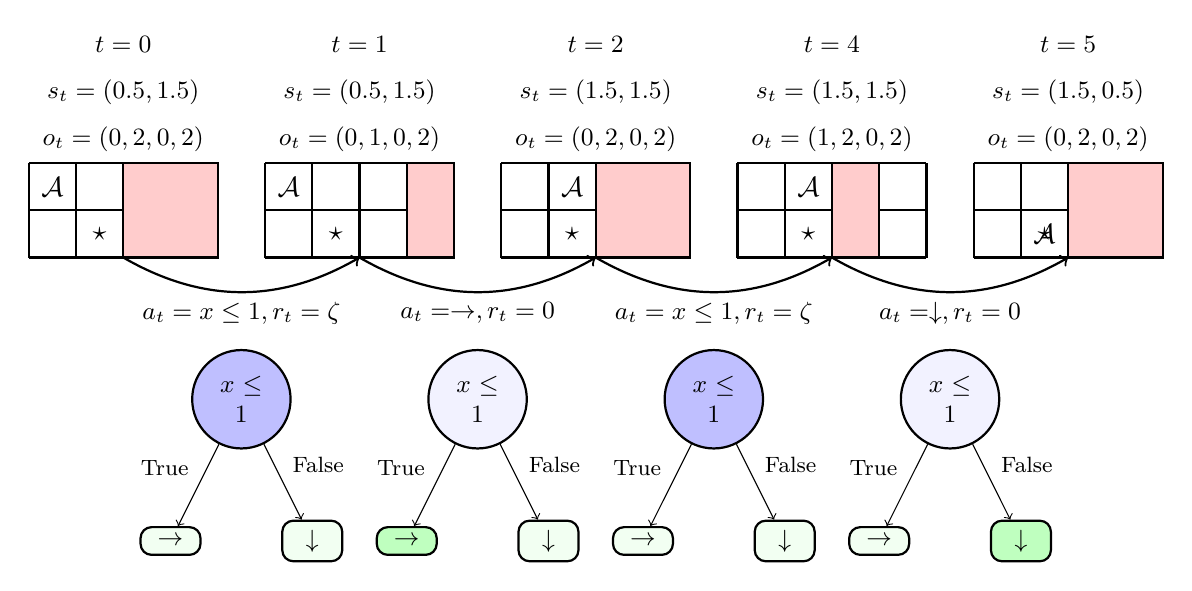
\begin{tikzpicture}[scale=0.6]
    % Define styles
    \tikzstyle{grid}=[draw, thick, fill=gray!10]
    \tikzstyle{rectangle}=[draw, thick, fill=red!20]
    
    % Row 1: IBMDP States (s, o)
    % t=0: Initial state
    \node at (2,8.5) {\small $t=0$};
    \node at (2,7.5) {\small $\boldsymbol{s}_t=(0.5, 1.5)$};
    \node at (2,6.5) {\small $\boldsymbol{o}_t=(0, 2, 0, 2)$};

    \draw[grid] (0,4) grid (2,6);
    \node at (0.5, 5.5) {$\mathcal{A}$};
    \node at (1.5, 4.5) {$\star$};

    \draw[rectangle] (2,4) rectangle (4,6);  
    
    % Curved arrow from t=0 to t=1
    \draw[thick, ->] (2,4) to[bend right=30] node[midway, below] {\small $a_t = x \leq 1, r_t = \zeta$} (7,4);

    % % t=1: After AIG x≤0.5
    \node at (7,8.5) {\small $t=1$};
    \node at (7,7.5) {\small $\boldsymbol{s}_t=(0.5, 1.5)$};
    \node at (7,6.5) {\small $\boldsymbol{o}_t=(0, 1, 0, 2)$};

    \draw[grid] (5,4) grid (7,6);
    \node at (5.5, 5.5) {$\mathcal{A}$};
    \node at (6.5, 4.5) {$\star$};

    \draw[grid] (7,4) grid (9,6);
    \draw[rectangle] (8,4) rectangle (9,6);

    % Curved arrow from t=1 to t=2
    \draw[thick, ->] (7,4) to[bend right=30] node[midway, below] {\small $a_t = \rightarrow, r_t  = 0$}(12,4);

    \node[circle, draw, thick, fill=blue!25, text width=2em, text centered, minimum height=1.5em, font=\small] (tree4_root) at (4.5,1) {$x \leq 1$};
    \node[rectangle, draw, thick, fill=green!5, text width=1.5em, text centered, rounded corners, minimum height=1em, font=\small] (tree4_right) at (3,-2) {$\rightarrow$};
    \node[rectangle, draw, thick, fill=green!5, text width=1.5em, text centered, rounded corners, minimum height=1em, font=\small] (tree4_left) at (6,-2) {$\downarrow$};
    \draw[->] (tree4_root) -- (tree4_right) node[font=\footnotesize, midway, above left] {True};
    \draw[->] (tree4_root) -- (tree4_left) node[font=\footnotesize, midway, above right] {False};

    \node at (12,8.5) {\small $t=2$};
    \node at (12,7.5) {\small $\boldsymbol{s}_t=(1.5, 1.5)$};
    \node at (12,6.5) {\small $\boldsymbol{o}_t=(0, 2, 0, 2)$};
    
    \draw[grid] (10,4) grid (12,6);
    \node at (11.5, 5.5) {$\mathcal{A}$};
    \node at (11.5, 4.5) {$\star$};
    \draw[rectangle] (12,4) rectangle (14,6);
    
    % Curved arrow from t=2 to t=4
    \draw[thick, ->] (12,4) to[bend right=30] node[midway, below] {\small $a_t = x \leq 1, r_t = \zeta$} (17,4);

    \node[circle, draw, thick, fill=blue!5, text width=2em, text centered, minimum height=1.5em, font=\small] (tree4_root) at (9.5,1) {$x \leq 1$};
    \node[rectangle, draw, thick, fill=green!25, text width=1.5em, text centered, rounded corners, minimum height=1em, font=\small] (tree4_right) at (8,-2) {$\rightarrow$};
    \node[rectangle, draw, thick, fill=green!5, text width=1.5em, text centered, rounded corners, minimum height=1em, font=\small] (tree4_left) at (11,-2) {$\downarrow$};
    \draw[->] (tree4_root) -- (tree4_right) node[font=\footnotesize, midway, above left] {True};
    \draw[->] (tree4_root) -- (tree4_left) node[font=\footnotesize, midway, above right] {False};

    
    \node at (17,8.5) {\small $t=4$};
    \node at (17,7.5) {\small $\boldsymbol{s}_t=(1.5, 1.5)$};
    \node at (17,6.5) {\small $\boldsymbol{o}_t=(1, 2, 0, 2)$};

    \draw[grid] (15,4) grid (17,6);
    \node at (16.5, 5.5) {$\mathcal{A}$};
    \node at (16.5, 4.5) {$\star$};
    \draw[grid] (17,4) grid (19,6);
    \draw[rectangle] (17,4) rectangle (18,6);
    
    \draw[thick, ->] (17,4) to[bend right=30] node[midway, below] {\small $a_t = \downarrow, r_t = 0$} (22,4);
    
    \node[circle, draw, thick, fill=blue!25, text width=2em, text centered, minimum height=1.5em, font=\small] (tree4_root) at (14.5,1) {$x \leq 1$};
    \node[rectangle, draw, thick, fill=green!5, text width=1.5em, text centered, rounded corners, minimum height=1em, font=\small] (tree4_right) at (13,-2) {$\rightarrow$};
    \node[rectangle, draw, thick, fill=green!5, text width=1.5em, text centered, rounded corners, minimum height=1em, font=\small] (tree4_left) at (16,-2) {$\downarrow$};
    \draw[->] (tree4_root) -- (tree4_right) node[font=\footnotesize, midway, above left] {True};
    \draw[->] (tree4_root) -- (tree4_left) node[font=\footnotesize, midway, above right] {False};


    \node at (22,8.5) {\small $t=5$};
    \node at (22,7.5) {\small $\boldsymbol{s}_t=(1.5, 0.5)$};
    \node at (22,6.5) {\small $\boldsymbol{o}_t=(0, 2, 0, 2)$};
 
    \draw[grid] (20,4) grid (22,6);
    \node at (21.5, 4.5) {$\mathcal{A}$};
    \node at (21.5, 4.5) {$\star$};
    \draw[rectangle] (22,4) rectangle (24,6);

    \node[circle, draw, thick, fill=blue!5, text width=2em, text centered, minimum height=1.5em, font=\small] (tree4_root) at (19.5,1) {$x \leq 1$};
    \node[rectangle, draw, thick, fill=green!5, text width=1.5em, text centered, rounded corners, minimum height=1em, font=\small] (tree4_right) at (18,-2) {$\rightarrow$};
    \node[rectangle, draw, thick, fill=green!25, text width=1.5em, text centered, rounded corners, minimum height=1em, font=\small] (tree4_left) at (21,-2) {$\downarrow$};
    \draw[->] (tree4_root) -- (tree4_right) node[font=\footnotesize, midway, above left] {True};
    \draw[->] (tree4_root) -- (tree4_left) node[font=\footnotesize, midway, above right] {False};

    

    
\end{tikzpicture}
\caption{An IBMDP trajectory when the base MDP is 2$\times$2 grid world, and equivalent decision tree policy traversal.
The pink obstructed squares represent the current bounds over state features. The more IGAs are taking, the more refined the bounds get.
At $t=0$, the state features are $\boldsymbol{s}_0 = (0.5, 1.5)$. 
The initial observation is always the base MDP default feature bounds, here $\boldsymbol{o}_0=(0, 2, 0, 2)$ because the base states are in $[0, 2] \times [0, 2]$.
The first action is an IGA that tests the feature $x$ of the states against the value $1$ and the reward $\zeta$. 
This transition corresponds to going through an internal node in a decision tree policy as illustrated in the figure. 
At $t=1$, after gathering the information that the $x$-value of the current base state is below 1, the observation is updated with the refined state bounds $\boldsymbol{o}_1=(0, 1, 0, 2)$ and the base state features remains unchanged. The agent then takes a base action that is to move right. 
This gives a reward 0, reinitialized the observation to the original bounds, and changes the base state to $\boldsymbol{s}_2=(1.5, 1.5)$. And the trajectory continues like this until the agent reaches the absorbing base state $\boldsymbol{s}_5=(1.5, 0.5)$.}
\label{fig:poibmdp_trajectory}
\end{figure}

\section{Summary}
In this chapter, we presented the approach of Topin et. al. (cite) to find trees that directly optimize the RL objective (cite) rather than the surrogate imitation loss.
To achieve that Topin et. al. showed that one can do RL of a partially observable deterministic policy for some IBMDP.

We can thus write an interpretable RL objective as follows:
\begin{definition}[Interpretable RL objective]
    Given a factored MDP $\mathcal{M}=\langle S, A, R, T, T_0 \rangle$, a discount factor $\gamma \in (0,1)$, and an associated IBMDP $\mathcal{M}_{IB}=\langle S \times O,A \cup A_{info}, (R, \zeta), (T_{info}, T, T_0)\rangle$, the goal of an interpetable RL agent is to find a partially observable IBMDP policy $\pi^\star_{po}:O\rightarrow A\cup A_{info}$ such that:
\begin{align*}
    \pi^\star_{po} &= \underset{\pi_{po}}{\opertarname{argmax}} \mathbb{E}\left[\sum_{t=0}^{\infty} \gamma^t R((\boldsymbol{s}_t, \boldsymbol{o}_t), a_t) \mid \boldsymbol{s}_0 \sim T_0, a_t = \pi_{po}(\boldsymbol{o}_t), \boldsymbol{s}_{t+1} \sim T(\boldsymbol{s}_t, a_t), \boldsymbol{o}_{t+1}\sim T(\boldsymbol{o_t}, a_t)\right]\\
    &= \underset{\pi_{po}}{\operatorname{argmax}} \mathbb{E}[V^{\pi}(s_0, o_0)| s_0\sim T_0]
\end{align*}
\end{definition}
In Figure (cite) we summarized the direct reinforcement learning approach of Topin et. al. that we use in the next chapters. 
\begin{figure}[h]
    \centering
    \begin{tikzpicture}
        \draw[fill=blue!30] (0, 0) rectangle (5.9, 3);
        \node at (3, 2.5) {IBMDP $\mathcal{M}_{IB} \langle \mathcal{M}, O, A_{info}, \zeta, T_{info}\rangle$};
        \draw[fill=blue!10] (0, 0) rectangle (5, 2);
        \node at (3, 1.5) {MDP $\mathcal{M} \langle S, A, R, T, T_0 \rangle$};
        
        \draw[fill=red!10] (10, 0) rectangle (14, 3);
        \node at (12, 2) {\textbf{Objective}};
        \node at (12, 1) {$\pi^{\star}_{po} = \underset{\pi_{po}}{\operatorname{argmax}} \mathbb{E}[V^{\pi_{po}}(\boldsymbol{s}_0, \boldsymbal{o}_0)| \boldsymbol{s}_0\sim T_0]$};
        
        \draw[fill=red!10] (1, -5) rectangle (5, -2);
        \node at (3, -3) {\textbf{Decision Tree Policy}};
        \node at (3, -4) {$\pi_{\mathcal{T}}: S \rightarrow A$};
        
        \draw[fill=red!10] (9.5, -5) rectangle (14.5, -2);
        \node at (12, -3) {\textbf{Deterministic Policy}};
        \node at (12, -4) {$\pi_{po}: O \rightarrow A \cup A_{info}$};
        
        \draw[thick, ->] (6, 2) -- (10, 2) node[midway, above] {$\gamma$};
        \draw[thick, <-] (5, -3.5) -- (9.5, -3.5) node[midway, above] {Extract tree with Alg 6};
        \draw[thick, ->] (12, 0) -- (12, -2) node[midway, left] {Solve with e.g. RL};
        \draw[thick, <-] (3, 0.5) -- (3, -2) node[midway, left] {Can be interpreted};
    
        
        % % Final arrow from tree back to base MDP - adjusted position
        % \draw[thick, ->] (1.75, -2.5) -- (1.75, -0.5) node[midway, right] {Can deploy\\and interpret};
        
    \end{tikzpicture}
    \caption{A formal framework to learn decision tree policies for MDPs. This include learning a partially observable deterministic policy in a POIBMDP (cite).}
    \label{fig:nested_decision_processes}
    \end{figure}

